%
%===============>>  Порядин Модуль 8 <<=============
%=
\setmodule{9}

%BEGIN_FOLD % ====>>_____ Занятие 1 _____<<====
\begin{class}[number=1]
	\begin{listofex}
		\item Вычислите:
		\begin{tasks}(2)
			\task \( ( 8 094 \cdot 4 + 24 592 : 8 ) - 24 869\)
			\task \( ( 63 725 + 41 375 - 103 228 ) : 4 \cdot 6 \)
			\task \( 13 257 + 4 326 : 7 \cdot 8 - 7 543 \)
			\task \( ( 60 000 - 32 216 + 54 674 ) : 9 \cdot 3 \)
			\task \( 847 \cdot 8 + ( 42 000 - 39 918) : 6 \)
			\task \( 602 630 - 297 480 : 37 \cdot 69 + 8 653 \)
		\end{tasks}
		\item Караван верблюдов шёл в первый день 8 ч со скоростью 9 км/ч, во второй день – 6 ч со скоростью 8 км/ч, а в третий день – 9 ч со скоростью 7 км/ч. Какое расстояние прошёл караван за 3 дня?
		\item Вертолёт пролетает 840 км за 3 ч, а автомобиль проходит это же расстояние за 7 ч. У кого из них скорость больше и на сколько?
		\item Поезд проходит 320 км за 5 ч. Какое расстояние он пройдёт за 8 ч, двигаясь с этой же скоростью?
		\item Туристы решили пройти за день 30 км. Они уже прошли 3 ч со скоростью 6 км/ч. Какое расстояние им осталось пройти?
		\item За сколько времени они пройдут это расстояние, двигаясь с прежней скоростью?
		\item Ира прошла 15 км за 3 ч, а Петя – 16 км за 4 ч. У кого из ребят скорость больше и на сколько?
		\item Автомобиль за 6 ч проехал 480 км. Какое расстояние мог бы проехать автомобиль за это же время, если бы увеличил скорость на 12 км/ч?
	\end{listofex}
\end{class}
%END_FOLD

%BEGIN_FOLD % ====>>_____ Занятие 2 _____<<====
\begin{class}[number=2]
	\begin{listofex}
			\item Караван верблюдов шёл в первый день 8 ч со скоростью 9 км/ч, во второй день --- 6 ч со скоростью 8 км/ч, а в третий день --- 9 ч со скоростью 7 км/ч. Какое расстояние прошёл караван за 3 дня?
		\item Вертолёт пролетает 840 км за 3 ч, а автомобиль проходит это же расстояние за 7 ч. У кого из них скорость больше и на сколько?
		\item Поезд проходит 320 км за 5 ч. Какое расстояние он пройдёт за 8 ч, двигаясь с этой же скоростью?
		\item Туристы решили пройти за день 30 км. Они уже прошли 3 ч со скоростью 6 км/ч. Какое расстояние им осталось пройти?
		\item За сколько времени они пройдут это расстояние, двигаясь с прежней скоростью?
		\item Ира прошла 15 км за 3 ч, а Петя --- 16 км за 4 ч. У кого из ребят скорость больше и на сколько?
		\item Автомобиль за 6 ч проехал 480 км. Какое расстояние мог бы проехать автомобиль за это же время, если бы увеличил скорость на 12 км/ч?
	\end{listofex}
\end{class}
%END_FOLD

%BEGIN_FOLD % ====>>_ Домашняя работа 1 _<<====
\begin{homework}[number=1]
	\begin{listofex}
		\item Вычислите:
		\begin{tasks}(2)
			\task \( (647\cdot 20 + 8232 : 3 ) - 67\)
			\task \( ( 7699 + 4561 - 3496 ) : 2 \cdot 4 \)
		\end{tasks}
		\item От города до посёлка автобус ехал \( 3 \) ч со скоростью \( 86 \) км/ч. Сколько времени понадобится самосвалу с грузом, чтобы проехать этот путь со скоростью \( 43 \) км/ч?
		\item Моторная лодка, двигаясь со скоростью \( 25 \) км/ч, прошла путь между пристанями за \( 2 \) ч. Сколько потребуется времени, чтобы пройти этот же путь на байдарке, если она движется со скоростью \( 5 \) км/ч?
		\item  Медуза плыла \( 2 \) ч со скоростью \( 50 \) м/ч и ещё \( 3 \) ч со скоростью \( 55 \) м/ч. Какой путь проплыла медуза?
		\item На лодке рыбаки плыли \( 2 \) ч со скоростью \( 4 \) км/ч. Оставшуюся часть пути они проплыли со скоростью \( 5 \) км/ч. На весь путь они затратили \( 5 \) ч. Какое расстояние проплыли рыбаки?
	\end{listofex}
\end{homework}
%END_FOLD

%BEGIN_FOLD % ====>>_____ Занятие 3 _____<<====
\begin{class}[number=3]
	\begin{listofex}
		\item  Автомобиль проехал первую часть пути за \( 2 \) ч со скоростью \( 82 \) км/ч. Оставшуюся часть пути он проехал за \( 3 \) ч. С какой скоростью ехал автомобиль оставшийся путь, если весь его путь равен \( 452 \) км?
		\item  Вертолёт пролетел \( 920 \) км за \( 4 \) ч. Какое расстояние он пролетит за \( 5 \) ч, если увеличит свою скорость на \( 60 \) км/ч?
		\item Первый пловец проплыл \( 100 \) м со скоростью \( 25 \) м/мин. Второй пловец потратил на эту дистанцию на \( 1 \) мин больше. С какой скоростью плыл второй пловец?
		\item Скорый поезд проехал \( 448 \) км со скоростью \( 56 \) км/ч, а на обратном пути это расстояние он проехал в \( 2 \) раза быстрее. За сколько часов проехал поезд весь путь туда и обратно?
		\item Из двух посёлков одновременно выехали навстречу друг другу велосипедист и мотоциклист. Они встретились через \( 4 \) ч. Скорость велосипедиста \( 15 \) км/ч, а мотоциклиста \( 57 \) км/ч. Чему равно расстояние между посёлками.
		\item От двух пристаней одновременно навстречу друг другу отошли катер и лодка. Они встретились через \( 6 \) ч. Скорость лодки \( 8 \) км/ч, а скорость катера \( 35 \) км/ч. Чему равно расстояние между пристанями.
		\item Два лыжника вышли одновременно навстречу друг другу из двух разных пунктов, расстояние между которыми \( 66 \) км. Скорость первого \( 12 \) км/ч. С какой скоростью ехал второй лыжник, если они встретились через \( 3 \) ч?
		\item Из двух городов одновременно навстречу друг другу выехали два мотоциклиста и встретились через \( 10 \) мин. Скорость одного из них \( 920 \) м/мин. Расстояние между городами \( 18 900 \) м. С какой скоростью ехал второй мотоциклист?
		\item Автомобиль и автобус выехали одновременно из двух городов навстречу друг другу. Скорость автомобиля \( 90 \) км/ч. Он проехал до встречи \( 900 \) км. Скорость автобуса \( 70 \) км/ч. Какое расстояние до встречи проедет автобус?
		\item От двух пристаней одновременно навстречу друг другу вышли два теплохода. Скорость первого \( 24 \) км/ч. Он прошёл до встречи \( 96 \) км. Второй теплоход шёл со скоростью \( 30 \) км/ч. Какое расстояние пройдёт до встречи второй теплоход?
	\end{listofex}
\end{class}
%END_FOLD

%BEGIN_FOLD % ====>>_____ Занятие 4 _____<<====
\begin{class}[number=4]
	\begin{listofex}
		\item  Из села выехал велосипедист, одновременно навстречу ему из города выехал мотоциклист. Велосипедист ехал со скоростью \( 12 \) км/ч, а мотоциклист в \( 5 \) раз быстрее, чем велосипедист. Они встретились через \( 4 \) ч. Каково расстояние между городом и селом?
		\item Две сёмги одновременно поплыли навстречу друг другу. Первоначальное расстояние между ними \( 158 \) км. Одна сёмга плыла со скоростью \( 39 \) км/ч, а другая на \( 1 \) км/ч быстрее. Через сколько часов они встретятся?
		\item Из своего гнезда одновременно в противоположных направлениях вылетели два осоеда. Один из них летел со скоростью \( 40 \) км/ч, а другой со скоростью \( 44 \) км/ч. Какое расстояние будет между ними через \( 3 \) ч?
		\item С одного аэродрома одновременно в противоположных направлениях вылетели два вертолёта. Скорость одного из них \( 243  \) км/ч, скорость другого на \( 18 \) км/ч меньше. Какое расстояние будет между ними через \( 3 \) ч?
		\item С турбазы вышли одновременно и пошли в противоположных направлениях два человека. Через \( 5 \) ч расстояние между ними было \( 45 \) км. Чему равна скорость второго человека, если первый человек шёл со скоростью \( 5 \) км/ч?
		\item Со стоянки одновременно отъехали в противоположных направлениях мотороллер и мотоцикл. Когда мотороллер проехал \( 90  \) км, расстояние между ними стало \( 455 \) км. Скорость мотороллера \( 18 \) км/ч. Найди скорость мотоцикла.
		\item  От пристани одновременно в противоположных направлениях отошли два катамарана. Скорость одного из них \( 15 \) км/ч, скорость другого на \( 2 \) км/ч меньше. Через какое время расстояние между ними будет \( 168 \) км?
		\item От одной пристани одновременно в противоположных направлениях отошли два теплохода со скоростью \( 35 \) км/ч и \( 39 \) км/ч. Какое расстояние прошёл каждый теплоход, когда расстояние между ними стало \( 222 \) км?
		\item Из одной деревни в другую направился велосипедист со скоростью \(  250  \) м/мин. Через \( 30 \) мин из другой деревни навстречу ему выехал второй велосипедист со скоростью \( 260 \) м/мин и встретил первого через \( 15 \) мин после своего выезда. Найди расстояние между деревнями.
		\item В школьной столовой молочный суп разлили в \( 18 \) тарелок. Это на \( 6 \) порции больше, чем рассольника. За обедом школьники съели \( 15 \) порций первого блюда. Сколько порций первых блюд осталось?
		\item Длина рулона белых обоев \( 16 \) м, а в рулоне коричневых обоев на \( 4 \) м меньше. Для ремонта квартиры купили \( 5 \) рулона белых обоев и \( 4 \) рулона коричневых. Сколько всего  метров обоев  купили для ремонта квартиры?
	\end{listofex}
\end{class}
%END_FOLD

%BEGIN_FOLD % ====>>_ Домашняя работа 2 _<<====
\begin{homework}[number=2]
	\begin{listofex}
		\item Гончая собака бежала \( 8 \) с со скоростью \( 30 \) м/с. На обратном пути то же расстояние собака пробежала за \( 12 \) с. Какова скорость собаки на обратном пути?
		\item Две девочки вышли одновременно навстречу друг другу из своих домов. Они встретились через \( 8 \) мин. Одна шла со скоростью \( 60 \) м/мин, а другая со скоростью \( 70 \) м/мин. Каково расстояние между домами девочек?
		\item Расстояние между сёлами \( 48 \) км. Из них вышли одновременно навстречу друг другу два пешехода. Скорость одного пешехода \( 3 \) км/ч. С какой скоростью шёл второй пешеход, если они встретились через \( 6 \) ч?
	\end{listofex}
\end{homework}
%END_FOLD

%BEGIN_FOLD % ====>>_____ Занятие 5 _____<<====
\begin{class}[number=5]
	\begin{listofex}
		\item Выполните деление:
		\begin{tasks}(3)
			\task \( 2380 : 14 \)
			\task \( 15436 : 68 \)
			\task \( 14168 : 46 \)
			\task \( 1814 : 49 \)
			\task \( 1495 : 23 \)
			\task \( 8658 : 74 \)
		\end{tasks} 
		\item Вычислите: \begin{tasks}(3)
			\task \( 84 000 : 1000  \)
			\task \( 5300 - 100   \)
			\task \(	207 000 : 10   \)
			\task \(	9400 - 10   \)
			\task \(	280- 100  \)
			\task \(	10 600 : 100 \)
		\end{tasks}
		\item Найдите значения выражений: \begin{tasks}(2)
			\task \( 672 : 8 + (801 - 204 \cdot 3) \)
			\task \( 430 - (701 000 : 1000 – 36 \cdot 10) \)
		\end{tasks}
		\item Решите уравнения: 
		\begin{tasks}(3)
			\task \( 83 - c = 52 \)
			\task \( 96 : a = 8  \)
			\task \( 6\cdot a : 12 = 11  \)
		\end{tasks}      
		\item Рабочий за 7-часовой рабочий день изготавливает 56 деталей, а его ученик за 4 ч в день изготавливает 24 такие детали. Сколько всего деталей изготавливают за 1 ч рабочий и его ученик вместе?
		\item Треугольник имеет следующие длины сторон: \( 4 \) см, \( 4 \) см и \( 4 \) см. Что это за треугольник?
		\item Какова площадь треугольника с основанием из \( 2 \) единиц и высотой \( 3 \) единицы?
		\item Найди периметр квадрата со сторонами \( 3 \) см \( 5 \) мм.
		\item Найди длину одной из сторон прямоугольника, если его площадь 18 см\( ^{2} \), а длина другой стороны 6 см.
		\item Длина участка земли прямоугольной формы \( 120 \) м, а ширина --- \( 30 \) м. Найди площадь участка земли.
		\item  Площадь крышки журнального столика прямоугольной формы \( 63 \) дм\( ^{2} \). Длина одной её стороны \( 9 \) дм. Найди периметр этого столика.
		\item Паша дразнил гуся на расстоянии \( 15 \) м, гуся разозлился и решил пощипать мальчика. Через сколько секунд гусь догонит Пашу, если Паша может пробежать за \(  44  \) секунды \( 262 \) метра, а гусь за \( 1 \) минуту \( 9 \) секунд пробегает \( 621 \) м?
		\item Вова и Неля играют в догонялки. Неля бегает со скоростью \( 4 \) м/с, а Вова может пробежать за \( 4 \) секунды \( 20 \) метров. Вова убегает от Нели --- какое расстояние будет между ними через \( 10 \) секунд?
		\item Участок земли для строительства санатория имеет форму прямоугольника, стороны которого равны \( 900 \) м и \( 400 \) м. Одна из больших сторон участка идёт вдоль моря, а три остальные стороны нужно отгородить забором. Найдите длину этого забора. Ответ дайте в метрах.
		\item 
		\begin{minipage}[t]{\bodywidth}
			Два садовода, имеющие прямоугольные участки размерами \( 35 \) м на \( 40 \) м с общей границей, договорились и сделали общий прямоугольный пруд размером \( 20 \) м на \( 14 \) м (см. чертёж), причём граница участков проходит точно через центр. Какова площадь (в квадратных метрах) оставшейся части участка каждого садовода?
		\end{minipage}
		\hspace{0.02\linewidth}
		\begin{minipage}[t]{\picwidth}
			% TODO: \usepackage{graphicx} required
			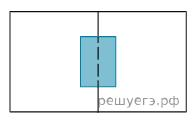
\includegraphics[align=t, width=\linewidth]{../../../../../exercises/lists/pics/poryadin4M9L5-3}
		\end{minipage}
	\end{listofex}
\end{class}
%END_FOLD

%BEGIN_FOLD % ====>>_____ Занятие 6 _____<<====
\begin{class}[number=6]
	\begin{listofex}
		\item Занятие 6
	\end{listofex}
\end{class}
%END_FOLD

%BEGIN_FOLD % ====>>_ Домашняя работа 3 _<<====
\begin{homework}[number=3]
	\begin{listofex}
		\item Вычислите:\begin{tasks}(2)
			\task \( 64: (4\cdot2)+14 \)
			\task \( 240+(620-200):7 \)
			\task \( 19\cdot3+27\cdot2\)
			\task \( 80\cdot3+450-90 \)
		\end{tasks}
		\item Два спортзала имеют одинаковую площадь. Ширина первого спортзала  \( 70 \) м, а ширина второго --- \( 60 \) м. Найди длину первого спортзала, если длина второго спортзала \( 140 \) м.
		\item Одна сторона четырёхугольника равна \( 48 \) см, вторая сторона на \( 14 \) см больше, чем первая, а третья сторона в \( 2 \) раза меньше суммы первых двух сторон. Найди четвёртую сторону, если периметр четырёхугольника равен \( 200 \) см.
	\end{listofex}
\end{homework}
%END_FOLD

%BEGIN_FOLD % ====>>_____ Занятие 7 _____<<====
\begin{class}[number=7]
	\begin{listofex}
		\item Расстояние между двумя посёлками \( 180 \) км рейсовый автобус проехал за \( 6 \) ч. На обратном пути его скорость увеличилась на \( 15 \) км/ч. Какое время рейсовый автобус потратил на весь путь туда и обратно?
		\item Машина шла до остановки \( 5 \) ч со скоростью \( 68 \) км/ч. После этого ей осталось проехать вдвое меньший путь, на который она потратила \( 2 \) ч. С какой скоростью ехала машина после остановки?
		\item Из двух городов навстречу друг другу одновременно выехали два мотоциклиста. Встретились они через \( 4 \) ч. Скорость одного мотоциклиста \( 85 \) км/ч, скорость другого \( 95 \) км/ч. Каково расстояние между городами?
		\item Два поезда вышли одновременно навстречу друг другу из двух городов, расстояние между которыми \( 650 \) км. Первый поезд ехал со скоростью \( 62 \) км/ч и проехал до встречи \( 310 \) км. С какой скоростью ехал второй поезд?
		\item Два поезда вышли из двух городов, расстояние между которыми \( 568 \) км, одновременно навстречу друг другу. Скорость первого поезда \( 68 \) км/ч, скорость второго \( 74 \) км/ч. Какое расстояние до встречи прошёл каждый поезд?
		\item С двух аэродромов одновременно вылетели навстречу друг другу два самолёта. Скорость первого самолёта \( 626 \) км/ч. Он пролетел до встречи \( 2504 \) км. Скорость второго самолёта \( 981 \) км/ч. Чему равно расстояние между аэродромами?
		\item Два мальчика вышли из своих домов, расстояние между которыми \( 480 \) м, одновременно навстречу друг другу. Первый мальчик шёл со скоростью \( 40 \) м/мин, а второй в \( 2 \) раза медленнее. Через сколько минут мальчики встретятся?
		\item От спортивной базы одновременно отъехали в противоположных направлениях два лыжника. Когда первый лыжник проехал \( 3645 \) м, расстояние между ними стало \( 7395 \) м. Скорость первого лыжника \( 243 \) м/мин. Найди скорость второго лыжника.
		\item Из одного города одновременно в противоположных направлениях выехали два мотоциклиста со скоростью \( 78 \) км/ч и \( 87 \) км/ч. Через какое время расстояние между ними будет \( 330 \) км?
	\end{listofex}
\end{class}
%END_FOLD

%BEGIN_FOLD % ====>>_____ Занятие 8 _____<<====
\begin{class}[number=8]
	\begin{listofex}
		\item \begin{tasks}(2)
			\task \( 12-3+4\cdot(3\cdot5-5) \)
			\task \( 6-2+3\cdot(2+45:8)-7+4\cdot4 \)
			\task \( (25-14)\cdot3-(21-3):9 \)
			\task \( 5\cdot10+4-13\cdot2-1 \)
			\task \( 36:4\cdot5+5-50 \)
			\task \( 23+84:(6\cdot7-12+9\cdot3\cdot2) \)
		\end{tasks}
		\item Паша дразнил гуся на расстоянии 15 м, гусь разозлился и решил пощипать мальчика. Через сколько секунд гусь догонит Пашу, если Паша может пробежать за 44 секунды 262 метра, а гусь за 1 мин 9 с пробегает 621 м?
		\item Вова и Неля играют в догонялки. Неля бегает со скоростью 
		4 м/с, а Вова может пробежать за 4 секунды 20 метров. Вова убегает от Нели - какое расстояние будет между ними 
		через 10 секунд?
		\item От двух пристаней навстречу друг другу одновременно вышли теплоход и катер. Теплоход шёл со скоростью 33 км/час, а катер --- 25 км/час. Через 3 часа они встретились. Чему равно расстояние между пристанями?
		\item Осьминог и каракатица испугались друг дружку и поплыли в разные стороны. Через 37 секунд между ними оказалось 2 516 дециметров. Сколько каракатица проплывает за 201 секунду, если осьминог плавает на 14 дм/с быстрее.
		\item  Из двух городов, расстояние между которыми 840 км, вышли одновременно навстречу друг другу 2 поезда. Скорость первого поезда --- 100 км/час, второго --- на 10 км/час больше. Через сколько часов поезда встретятся?
	\end{listofex}
\end{class}
%END_FOLD

%BEGIN_FOLD % ====>>_____ Домашняя работа 4 _____<<====
\begin{homework}[number=4]
	\begin{listofex}
		\item Вычислите:
		\begin{tasks}(2)
			\task \( 2056 + 5435 : 5 - 234 \)
			\task \( 5931 - 31\cdot 4 + 538 \)
			\task \( 9522 + 6213\cdot 3 - 156 \)
			\task \( 3657 - 561 \cdot 3 - 853 \)
			\task \( 454 + 4872 : 3 + 643 \)
			\task \( 1090 + 3456: 4 + 8979 \)
		\end{tasks}
		\item Масса восьми одинаковых ящиков с черносливом равна 100 кг. Масса пустого ящика равна 500 грамм. Чему равна масса чернослива в одном ящике?
	\end{listofex}
\end{homework}
%END_FOLD